\section{Réseaux récurrents}
\label{recarchi}
\subsection{Généralités théoriques}
% https://arxiv.org/pdf/1801.01078.pdf
\subsubsection{Description d'un RNN}
\noindent Les architectures neuronales populaires (tels que les réseaux convolutifs ou les réseaux Full-Connected) ne possèdent pas une mémoire de leurs états internes. Ainsi, pour chaque donnée, ces réseaux ne considèrent pas le contexte de la donnée traitée et traitent chaque entrée indépendamment les unes des autres. En d'autres mots, ces réseaux reposent sur l'\textbf{hypothèse forte} que chaque donnée sont indépendantes.\\

\noindent Bien que possiblement vraie, dans les faits, cette condition est rarement vérifiée. Souvent négligeable, notamment dans le cadre de l'analyse d'image, elle est critique lorsque la donnée possède une forte liaison avec son contexte. C'est le cas pour toute donnée sérielle ou temporelle, tout particulièrement les données textuelles qui possèdent un fort potentiel applicatif (traduction automatique, reconnaissance vocale, commentaire/labellisation d'image...).\\

\noindent De plus, ces architectures imposent que la dimension d'entrée et de sortie soit fixe, ce qui est problématique dans le cadre d'analyse de données à dimension variable caractéristiques des données textuelles. Pour répondre à cette problématique, les \textit{réseaux récurrents}\cite{rnn} (RNNs - Reccurent Neural Network) ont été crées.\\

\noindent Contrairement aux autres architectures, un RNN possède une mémoire de ses états précédents. De ce fait, un RNN évalue une donnée à l'instant $t+1$ selon ses caractéristiques et son contexte représenté par le comportement du réseau vis-à-vis de la donnée $x_{-1},...,x_{-t}$ à l'instant $t,...,0$. La mémoire est caractérisée par une connexion entre chacune des cellules du RNN permettant la propagation de l'état caché qui représente le contexte informatif.\\

\noindent L'idée principale d'un RNN est de compresser l'information d'une séquence d'entrée en un vecteur $k \in R^d$ par récursivité. Ce vecteur est appelé \textit{état caché} et résume l'information, à l'instant t, du signal traité (représenté par l'ensemble des données $x_0,...,x_t$ analysées). Ainsi, à l'instant t, un \textit{état caché} possède une connaissance liée à la donnée $x_t$ et de son contexte défini par les données $x_{t-1},...,x_0$. L'\textit{état caché} obtenu à l'instant t est ensuite transmis à la cellule $t+1$ du RNN pour participer à la création de l'\textit{état caché} $t+1$ qui possédera l'information des données $x_0,...,x_t$ complétée par celle de la données $x_{t+1}$. L'\textit{état caché} à l'instant t est exploité pour réaliser la prédiction du RNN à l'instant t.\\

\noindent Il est \textbf{important} de retenir que chaque cellule d'un RNN sont strictement identiques. Les seules variables sont définies par les entrées i.e l'état caché et la donnée de l'instant t. Une illustration d'un RNN est visible sur la Figure \ref{RNNunrolled}. On peut observer une version unitaire et déroulée. Cette double représentation est possible car il y a unicité de l'architecture et des vecteurs de poids de chaque cellule.\\

\begin{figure}
\centering
    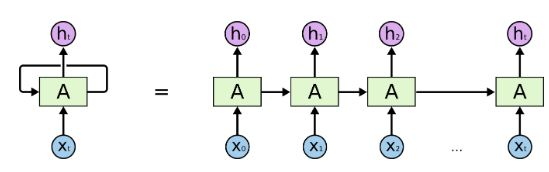
\includegraphics[scale=0.5]{./tex/recurrent-neural-network/rnn.jpg}
    \caption{Représentation d'un RNN "déroulé" allant de l'instant $0$ à $t$.}
    \label{RNNunrolled}
\end{figure}

\noindent \textbf{Remarque}: Un état de l'Art avancé a été réalisé par Hojjat Salehinejad sur l'architecture RNN. Il est consultable via son article de recherche \cite{rnn_news}. Cet article permet d'avoir une vision d'ensemble de l'évolution de l'architecture RNN, notamment de ces innovations les plus récentes.

\subsubsection{Présentation théorique}
\noindent Soit X une séquence, $X_1$, $X_2$, ... $X_t$ les éléments de cette séquence tels que $X = (X_1, ..., X_t)$. Soit $h_t$ l'état caché du RNN à l'instant $t$ et $y_t$, la prédiction du RNN à l'instant $t$ alors:
$$h_t = \sigma_h(U_{hX}X_t + W_{hh} h_{t-1} + b_h)$$
$$y_t = \sigma_y(V_{yh}h_t + b_y)$$

\noindent Avec U, matrice de poids de dimension $h \times X$\footnote{Prends en entrée une donné de dimension X et produit un résultat de dimension h}, $W_{hh}$ matrice de poids de dimension $h \times h$, V, matrice de dimension $y \times h$, $b_h$ et $b_y$, biais des couches et $\sigma$, fonction d'activation. Par convention, $\sigma_h$ correspond à la fonction tanh ou ReLU et $\sigma_y$, fonction sigmoïde ou softmax selon le type de prédiction réalisée. Une illustration est visible sur la Figure \ref{RNNdetails}.\\

\begin{figure}[h]
    \centering
    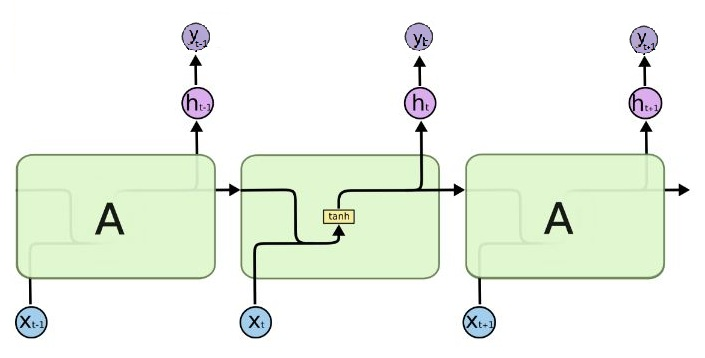
\includegraphics[scale=0.5]{./tex/recurrent-neural-network/rnndetail.jpg}
    \caption{Exemple d'une cellule RNN.}
    \label{RNNdetails}
\end{figure}

\noindent La dimension de l'état caché est de dimension fixe à travers le réseau et ce dernier est initialisé comme vecteur nul par convention à l'étape $t=0$.\\

\noindent Ce type de cellule est appelé \textit{Réseau de Helman}. Il existe de nombreuses variantes de cellule notamment le \textit{Réseau de Jordan} défini par:
$$h_t = \sigma_h(U_{hX}X_t + W_{hh} y_{t-1} + b_h)$$
$$y_t = \sigma_y(V_{yh}h_t + b_y)$$

\noindent Ces deux architectures sont très similaires. La différence repose sur le vecteur propagé entre les cellules. Dans le cas de Helman, il s'agit de l'état caché. Dans le cas de Jordan, du vecteur de sortie de la cellule. L'approche de Jordan, en n'exploitant pas l'état caché, perd le contexte général de la séquence et se focalise exclusivement sur le contexte $t-1$. En pratique, notamment les \textit{Neural Machine Translation}, les deux vecteurs sont exploités afin d'obtenir un compromis entre contexte proche et contexte global. \\

\subsubsection{Implémentation et représentation matricielle}
En cours
% Citer la partie \ref{matricie_calcul_nn}
\subsubsection{Apprentissage d'un RNN}

\subsubsection{Problématiques d'un RNN Vanilla}

\noindent Bien que théoriquement efficace\footnote{Un RNN est une architecture Turing complete \cite{rnn_turing}}, l'architecture RNN Vanilla présente des problèmes majeurs qui nuisent à son efficacité applicative.

\paragraph{Unilatéralité du contexte}

\noindent Un RNN, à l'instant t, exploite l'information à l'instant $[0,...,t-1,t]$. De ce fait, il ne possède qu'une vision unidirectionnelle pour réaliser sa prédiction. Ceci est très problématique car il biaise le contexte qui ne considère pas une direction informative.\\

\noindent Supposons une séquence $[x_0,...x_t,...,x_n]$. A l'instant t, la prédiction réalisée dépendra de $[x_0,...,x_t]$. Les valeurs $x_{t+1},...x_n$ ne sont donc pas considérées pour définir le contexte de la prédiction $y_t$. Ce défaut est critique dans le cadre du \textit{Natural Language Processing} car le contexte d'une phrase (ou plus spécifiquement d'un mot) s'étend sur l'ensemble de la séquence considérée\footnote{Cette affirmation est générale mais dépend grandement de la langue étudiée. En effet, la structure grammaticale varie grandement d'une langue à une autre.}. Pour répondre à cette problématique, les \textit{Réseaux récurrents bidirectionnels}\footnote{Bien qu'expérimentalement efficace, cette méthode est parfois considérée comme une méthode "cache-misère"...} ont été proposés.

\paragraph{Mémoire court terme}

\noindent Le vecteur de contexte (l'état caché) résume l'information de la séquence déjà observée. Dans les faits, l'information retenue est très peu uniforme et se concentre sur les dernières données observées. La Figure \ref{rnn_vanishing} illustre ce phénomène. Ainsi, un RNN possède essentiellement une mémoire à \textbf{court terme} et ceci est très néfaste dans le cadre d'analyse de séquences longues telles les textes ou encore les données temporelles. Pour corriger ce défaut, de nouvelles architectures de cellules ont été proposées, notamment les LSTM (\textit{Long Short-Term Memory}) et les GRU (\textit{Gated Reccurent Unit}).

\begin{figure}
    \centering
    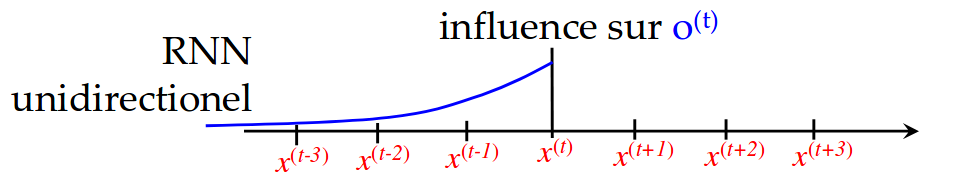
\includegraphics[scale=0.3]{./tex/recurrent-neural-network/rnn_vanish.png}
    \caption{Influence de la donnée selon sa position dans la séquence}
    \label{rnn_vanishing}
\end{figure}

\paragraph{Coût Calcul et représentativité de l'état caché}

\noindent L'état caché d'une cellule RNN est de dimension fixée (supposons de dimension d) et constante. De ce fait, une hypothèse forte est faite en supposant qu'un espace de dimension d est capable de représenter le phénomène observé. Une dimension trop grande favoriserait un sur-apprentissage\footnote{Apprendre par coeur chaque exemple, ce qui serait critique pour la généralisation du modèle} alors qu'une dimension trop petite ne permettrait pas la représentation de l'information utile de la donnée observée. Le choix de la dimension de l'état caché est un hyperparamètre qui peut être difficile à réaliser. Des valeurs \textit{par défaut} ont été proposées dans le cadre d'études empiriques mais il reste difficile de \textit{définir} une bonne valeur pour un problème donné. \\

\noindent Le problème de la dimension de l'état caché est directement lié au coût calcul d'une architecture RNN. Du fait du comportement séquentiel de ce type de réseau, ce dernier ne peut pas être efficacement parallélisé. Ainsi, les RNN sont des architectures coûteuses en temps machine (notamment pour l'apprentissage). Exploiter une dimension faible pour représenter l'état caché favorise une plus grande vélocité au risque d'une perte d'efficacité. Le choix de la dimension est donc un compromis entre \textit{Représentativité}, \textit{Généralisation} et \textit{Optimisation calculatoire}.


\subsection{Long Short-Term Memory (LSTM) - A FAIRE}
En cours
\subsection{Gated Recurent Unit (GRU) - A FAIRE}
En cours
\subsection{BiRNN - A FAIRE}
En cours
\subsection{Architecture-type}
Du fait du comportement sérielle de l'architecture récurrente, plusieurs variantes sont réalisables:\\

\begin{itemize}
    \item \textbf{One-to-One}: Cette architecture est la plus simple et correspond à un réseau récurrent composé d'une cellule uniquement. Ainsi, pour une entrée, le réseau produit une sortie.\\

    \item \textbf{One-to-Many}: Cette architecture prend en entrée une valeur unitaire et produit une sortie multiple. Elle est exploitée lors d'une tâche de prédiction d'un phénomène sériel à partir d'une valeur donnée (série temporelle par exemple). Dans le cas où l'on veut prédire les valeurs t+1,...,t+n, il faudrait un réseau One-to-N.\\

    \item \textbf{Many-to-One}: Cette architecture est l'inverse du \textit{One-to-Many}. A partir d'un ensemble sériel, on cherche à prédire une unique valeur. On peut exploiter cette approche lorsque l'on veut prédire une valeur t+1 à partir d'un contexte formé des valeurs t-n,...t.\\

    \item \textbf{Many-to-Many}: Cette architecture est caractéristique d'un \textit{Encoder-Decoder}. L'objectif est de prédire une succession d'états à partir d'une succession d'états. La dimension de l'entrée peut être différente de la dimension de sortie (M-to-N). Cette architecture est à la base des modèles de \textit{Natural Machine Translation} car elle permet de s'émanciper de la contrainte de la continuité dimensionnelle entre l'entrée et la sortie (i.e N=M).\\

    \item \textbf{Many-to-Many stricte}: Cette architecture est identique au \textit{Many-to-Many} mais impose une continuité dimensionnelle entre le signal d'entrée et le signal de sortie. Cette approche est souvent représentée comme la version naïve du \textit{Many-to-Many}, notamment pour les tâches de traduction.
\end{itemize}

\noindent Les différentes architectures sont illustrées sur la Figure \ref{archirec}. Elles sont indépendantes de la structure de la cellule choisie (LSTM, GRU ou RNN vanilla).
\begin{figure}
    \centering
    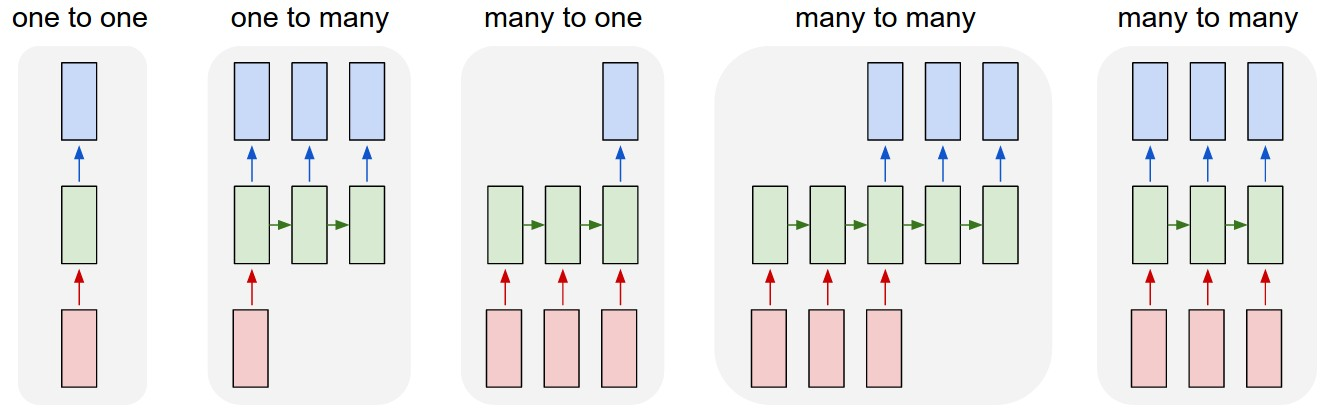
\includegraphics[scale=0.3]{./tex/recurrent-neural-network/archirec.jpg}
    \caption{Architecture-type d'un réseau récurrent}
    \label{archirec}
\end{figure}
